\documentclass[11pt]{article}
\usepackage{graphicx, amsmath, amssymb,enumerate,listings}
\usepackage[height=9in,width=7in]{geometry}
\usepackage{url}
\usepackage{tikz}
\usetikzlibrary{trees}
\usepackage{tikz}
\usepackage{graphicx, amsmath, amssymb,enumerate,listings}
\usepackage[height=9in,width=7in]{geometry}
\usetikzlibrary{automata,positioning}

\begin{document} 
\noindent
CSC420Assignment 1 \\
By: Ou Ye 999768327\\

\noindent
\textbf{1.a} 
\begin{lstlisting}[
  mathescape,
  columns=fullflexible,
  basicstyle=\fontfamily{ttdefault}\selectfont,
]
function finalImage = myconv(inputImage, filter) 

    imageSize = size(inputImage);
    finalImage = zeros(imageSize(1), imageSize(2), 'single');

    for  x = 1:imageSize(1)
        for  y = 1:imageSize(2)
            finalImage(x, y) = myconvHelper(inputImage, rot90(filter,2), x, y, imageSize(1), imageSize(2));
        end
    end
end

function computedValue = myconvHelper(imageMatrix, filter, x, y,xUpperBound, yUpperBound) 

    computedValue = 0;
    filterSize = size(filter);
    filterMedian = ceil(filterSize(1) / 2);
   
    for  x2 = 1:filterSize(1)
        for  y2 = 1:filterSize(2)
            
            x3 = (x - (x2 - filterMedian));
            y3 = (y - (y2 - filterMedian));

            if (x3 > 0 && y3 > 0 && x3 <= xUpperBound && y3 <= yUpperBound) 
                test1 = filterSize(1) - x2 + 1;
                test2 = filterSize(1) - y2 + 1;
                tempValue = double(imageMatrix(x3, y3))*double(filter(test1, test2));
                computedValue = double(computedValue) + tempValue;
            end
        end
    end
    
    computedValue = ceil(computedValue);
end
\end{lstlisting}

\noindent
\textbf{1.b} \\
Yes, it is possible to write a convolution in one pixel as a dot product between two vectors through the equation below. \\\\
It is also how the algorithm works in 1.a by computing the dot product for each and every pixel one at a time.\\
$$G[i,j] = \sum_{u=-k}^{k}\sum_{v=-k}^{k}h[u,v]F[i - u, j -u]$$\\

\noindent
Yes, it is possible to write the full convolution between the image and the filter via matrix multiplication.\\

\noindent
\textbf{2.a} \\
Given a $n * n$ image I, and $m * m$ filter h\\
The computational cost of computing the convolution is
$$Cost = h * I = m^2$$ 
based on lecture2.pdf slide 50 \\

\noindent
The computational cost if h is a separable filter is\\
$$Cost = h_x * I + h_y * I = 2m$$
based on lecture2.pdf slide 50 \\

\noindent
\textbf{2.b} \\
No, because from lecture2.pdf slide 49, we know that \\
Convolving twice with Gaussian kernel of width $\sigma$ is the same as convolving \\
once with kernel of width $\sigma \sqrt{2}$, therefore,
$$\sigma \sqrt{2} \neq \sigma$$ \\

\noindent
\textbf{2.c} 
\begin{lstlisting}[
  mathescape,
  columns=fullflexible,
  basicstyle=\fontfamily{ttdefault}\selectfont,
]
function resultImage = anisotropicGaussianFilter(inputImage, sigmaX, sigmaY) 

    h_x = uint8(fspecial('gaussian', [1 15*sigmaX], sigmaX)*255); 
    h_y = uint8(fspecial('gaussian', [15*sigmaY 1], sigmaY)*255); 

    resultImage = conv2(double(inputImage), double(h_x), 'same');
    resultImage = conv2(double(resultImage), double(h_y), 'same');
    
end
\end{lstlisting}
\newpage
\noindent
\textbf{2.d} \\
Using anisotropicGaussianFilter from 2c \\
\begin{lstlisting}[
  mathescape,
  columns=fullflexible,
  basicstyle=\fontfamily{ttdefault}\selectfont,
]
cat = rgb2gray(imread('./cat.jpg'));
figure;
imshow(anisotropicGaussianFilter(cat, 15, 2), []);
\end{lstlisting}

\begin{figure}[h]
  \caption{The result image after convolved with Gaussian filter with $\sigma_x = 15$
and $\sigma_y = 2$ }
  \centering
    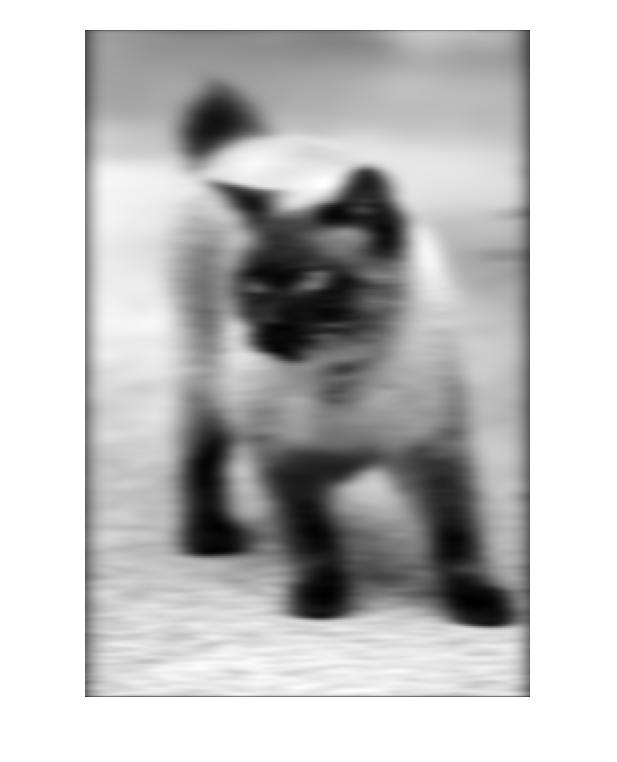
\includegraphics[width=0.5\textwidth]{2d}
\end{figure}




\noindent
\textbf{2.e} \\
If the Gaussian filter in question 2.d is separable, then we know we can decompose the Gaussian filter h of size $m*m$ into 2 smaller filters called $h_x$, and $h_y$ of size m. \\

\noindent
Then, convolve the input image with $h_x$ and convolve the output again with $h_y$ to obtain the final blur image, which is equivalent  of convolving the Gaussian filter h with the image. But because each $h_x, h_y$ is only size m, it only takes m operations to convolve where as it takes $m^2$ operations to convolve the filter h directly on the image.\\  

\noindent
Hence, it takes total of 2m operations to convolves for $h_x, h_y$, and $m^2$ for h.\\


\newpage
\noindent
\textbf{3.a} 
\begin{lstlisting}[
  mathescape,
  columns=fullflexible,
  basicstyle=\fontfamily{ttdefault}\selectfont,
]
templateNoise = rgb2gray(imread('./templateNoise.png'));
waldoNoise = rgb2gray(imread('./waldoNoise.png'));

% Template Noise
templateNoiseSigma1 = findGradient(templateNoise, 1);
templateNoiseSigma2 = findGradient(templateNoise, 2);
templateNoiseSigma3 = findGradient(templateNoise, 3);

imshow(templateNoiseSigma1, [])
figure
imshow(templateNoiseSigma2, [])
figure
imshow(templateNoiseSigma3, [])

% WaldoNoise
waldoNoiseSigma1 = findGradient(waldoNoise, 1);
waldoNoiseSigma2 = findGradient(waldoNoise, 2);
waldoNoiseSigma3 = findGradient(waldoNoise, 3);

figure
imshow(waldoNoiseSigma1, [])
figure
imshow(waldoNoiseSigma2, [])
figure
imshow(waldoNoiseSigma3, [])

function gradient = findGradient(inputImage, gaussianSize) 

    filterX = [
        -1 0 +1; ...
        -2 0 +2; ...
        -1 0 +1;
        ];

    filterY = [
        -1 -2 -1; ...
        0 0 0; ...
        1 2 1;
        ];

    blurImage = imgaussfilt(inputImage, gaussianSize);
    gX = conv2(double(blurImage), double(filterX), 'same');
    gY = conv2(double(blurImage), double(filterY), 'same');

    gradient = sqrt(double(gX).^2 + double(gY).^2);
end
\end{lstlisting}
\noindent
\textbf{3.a} 
\begin{figure}[h]
  \caption{TemplateNoise.jpg at $\sigma = 1, 2, 3$ }
    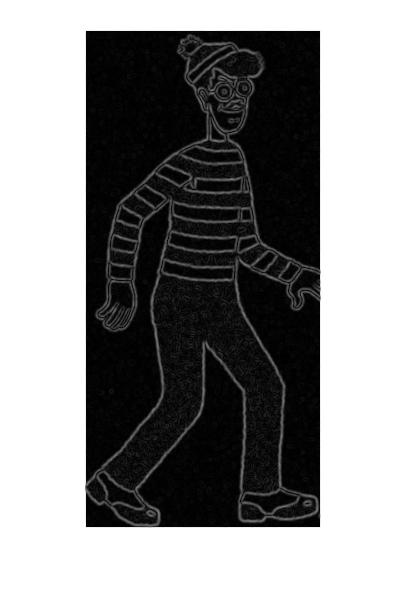
\includegraphics[width=0.34\textwidth]{templateNoiseSigma1}
    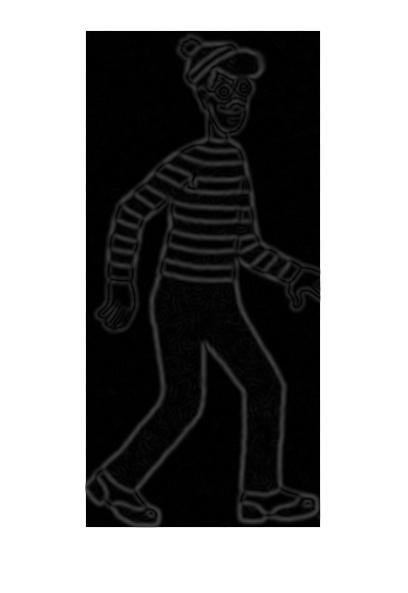
\includegraphics[width=0.34\textwidth]{templateNoiseSigma2}
    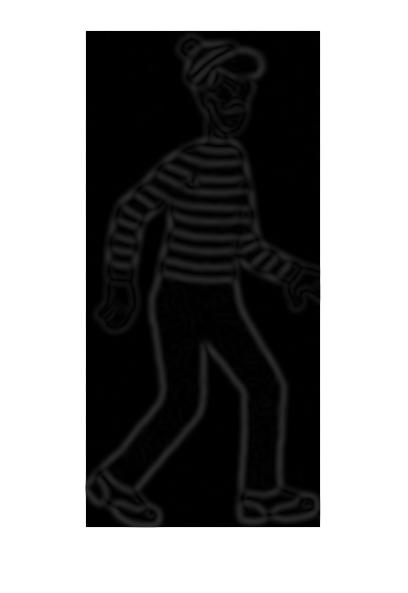
\includegraphics[width=0.34\textwidth]{templateNoiseSigma3}
\end{figure}

\begin{figure}[h]
  \caption{waldNoises.jpg at $\sigma = 1, 2, 3$ }
    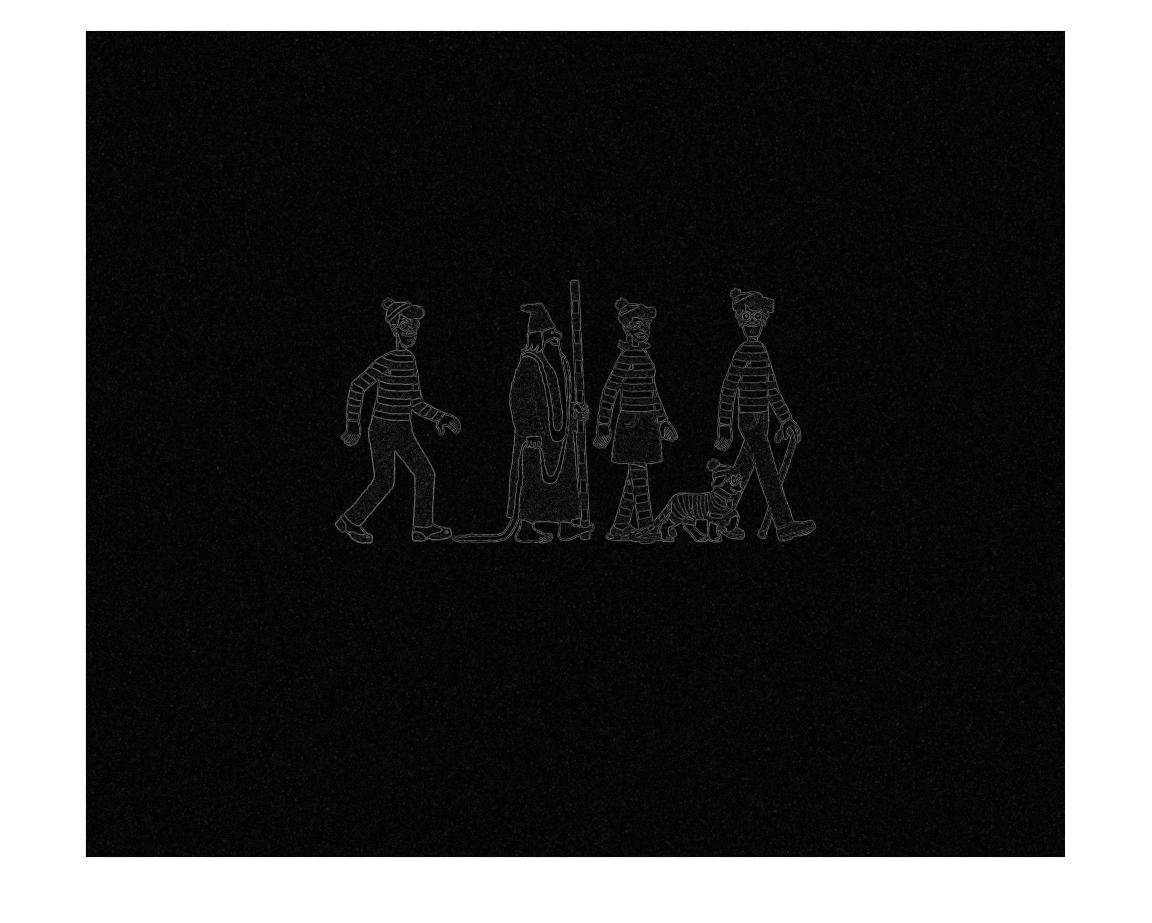
\includegraphics[width=0.34\textwidth]{waldoNoiseSigma1}
    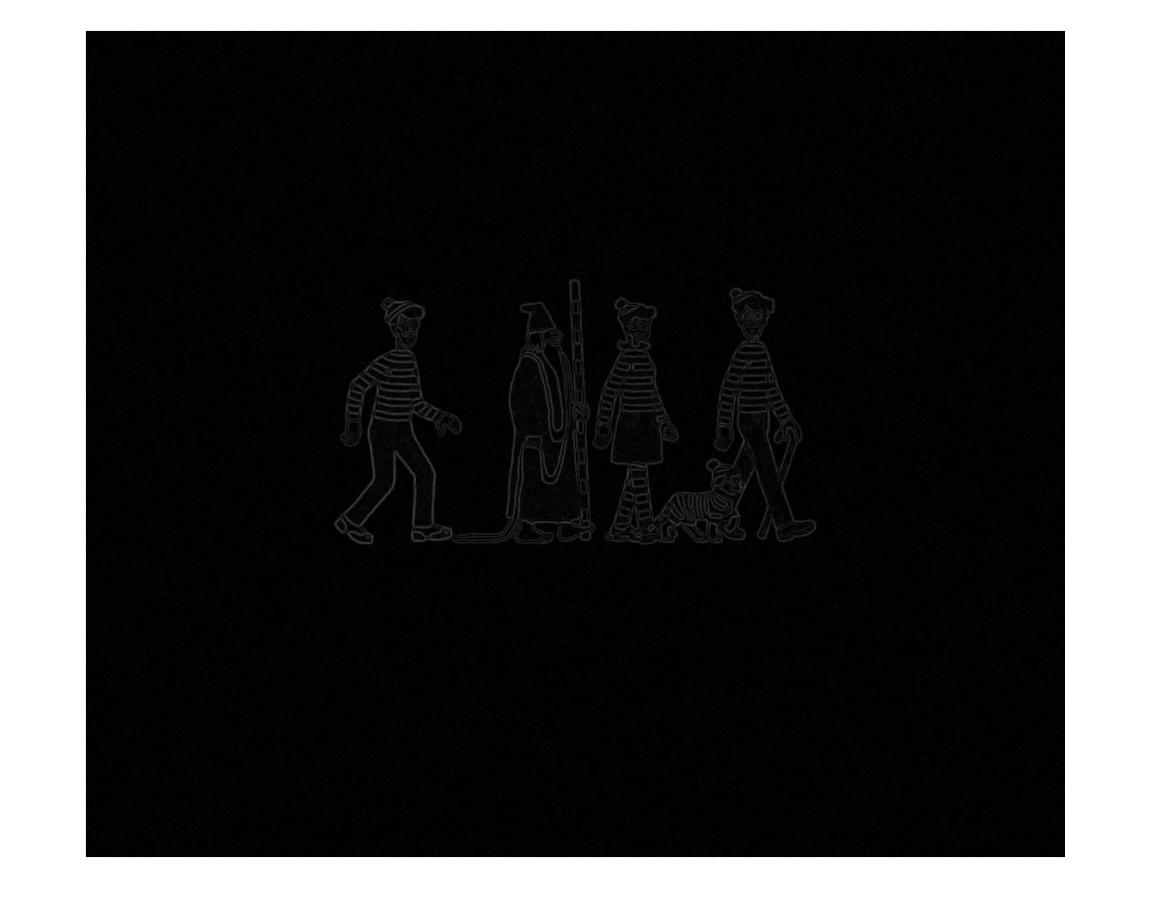
\includegraphics[width=0.34\textwidth]{waldoNoiseSigma2}
    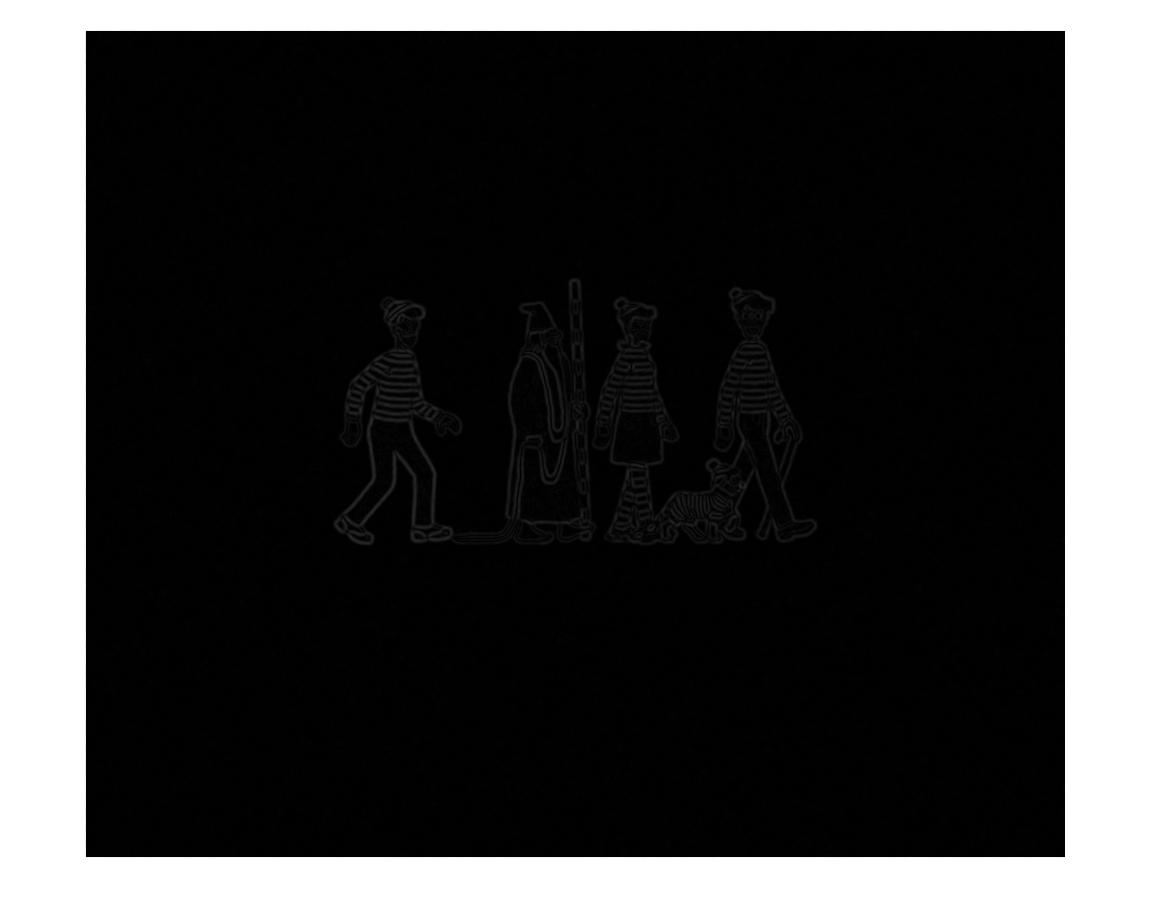
\includegraphics[width=0.34\textwidth]{waldoNoiseSigma3}
\end{figure}

\newpage
\noindent
\textbf{3.b} 
\begin{lstlisting}[
  mathescape,
  columns=fullflexible,
  basicstyle=\fontfamily{ttdefault}\selectfont,
]
templateNoise = rgb2gray(imread('./templateNoise.png'));
waldoNoise = rgb2gray(imread('./waldoNoise.png'));

templateNoiseSigma1 = findGradient(templateNoise, 1);
waldoNoiseSigma1 = findGradient(waldoNoise, 1);
result = findWaldo(waldoNoiseSigma1, templateNoiseSigma1);

function out = findWaldo(im, filter)
% returns the output of normalized cross-correlation between image im and
% filter 
% by Sanja Fidler, UofT
% convert image (and filter) to grayscale
im_input = im;
%im = rgb2gray(im);
im = double(im);
%filter = rgb2gray(filter);
filter = double(filter);
filter = filter/sqrt(sum(sum(filter.^2)));

% normalized cross-correlation
out = normxcorr2(filter, im);

% plot the cross-correlation results
figure('position', [100,100,size(out,2),size(out,1)]);
subplot('position',[0,0,1,1]);
imagesc(out)
axis off;
axis equal;

% find the peak in response
[y,x] = find(out == max(out(:)));
y = y(1) - size(filter, 1) + 1;
x = x(1) - size(filter, 2) + 1;

% plot the detection's bounding box
figure('position', [300,100,size(im,2),size(im,1)]);
subplot('position',[0,0,1,1]);
imshow(im_input, [])
axis off;
axis equal;
rectangle('position', [x,y,size(filter,2),size(filter,1)], 'edgecolor', [0.1,0.2,1], 'linewidth', 3.5);

end
\end{lstlisting}
\newpage

\noindent
\textbf{3.b} 
\begin{figure}[h]
  \caption{waldoNoise.jpg Gradient magnitude with $\sigma_1$}
  \centering
    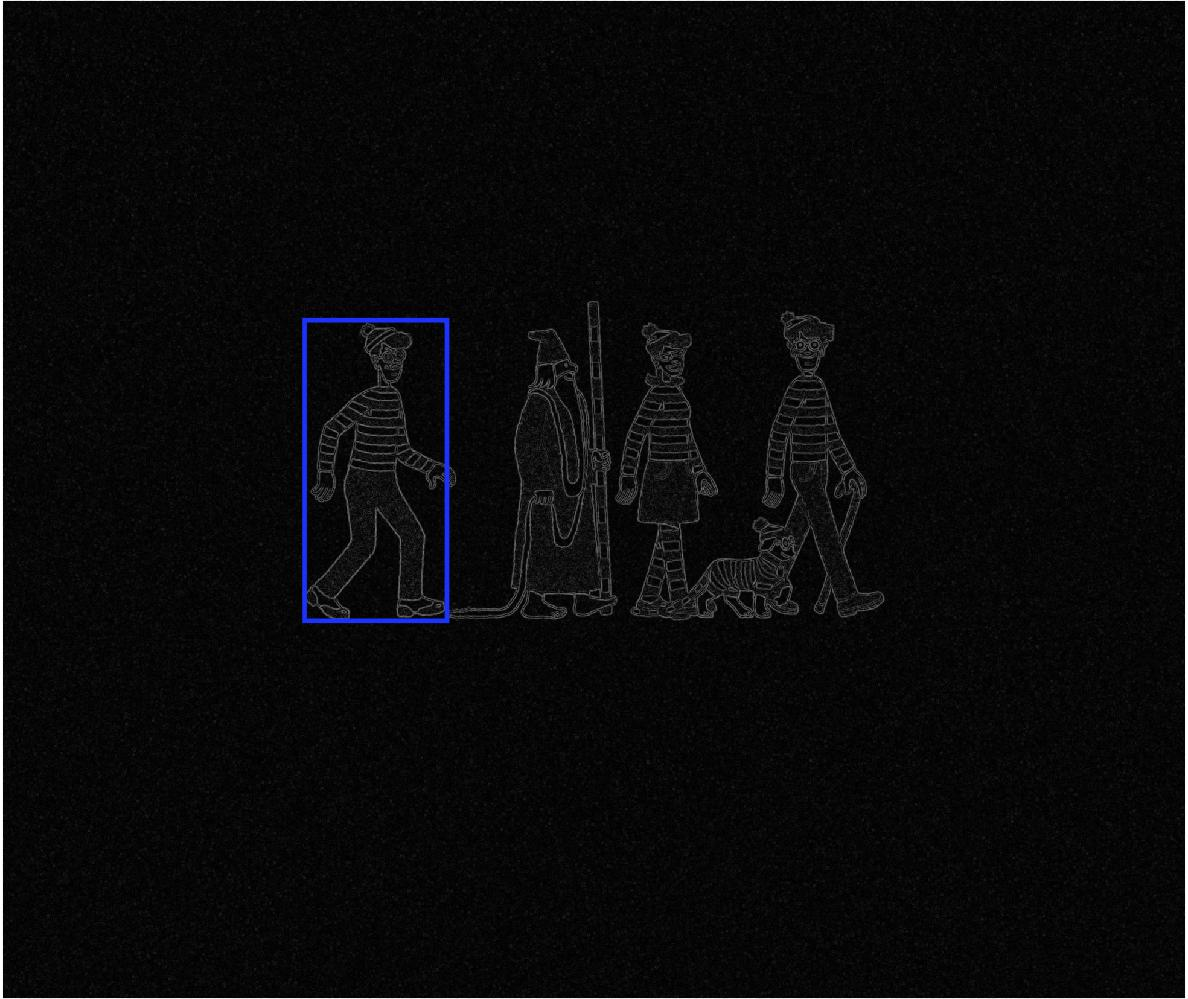
\includegraphics[width=0.5\textwidth]{3b}
\end{figure}

\begin{figure}[h]
  \caption{The cross correlation between waldoNoiseSigma1 and templateNoiseSigma1}
  \centering
    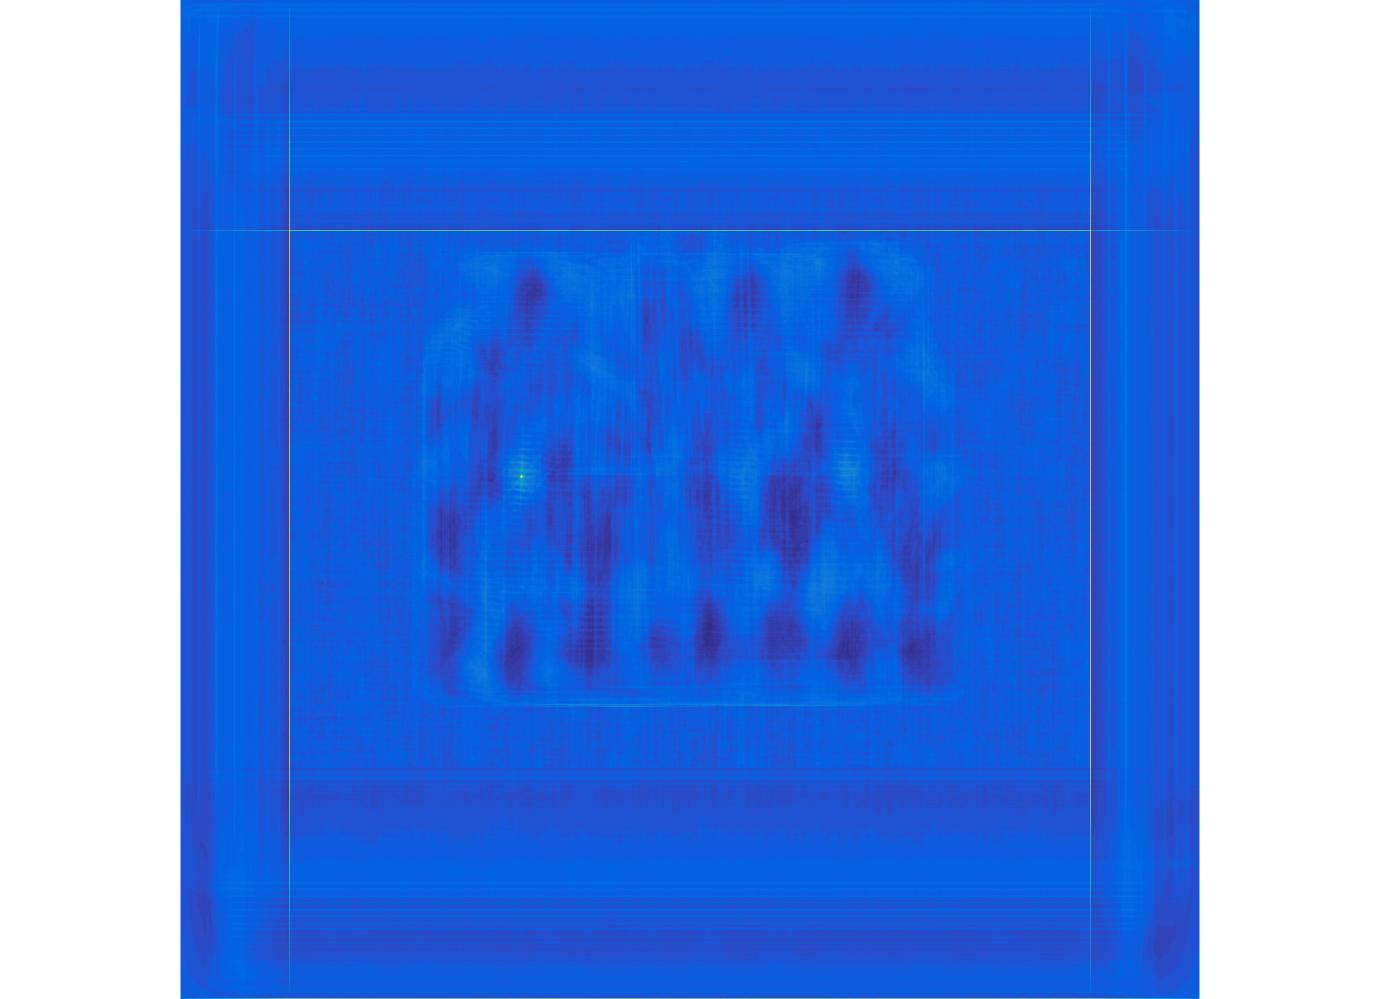
\includegraphics[width=0.6\textwidth]{3bCorr}
\end{figure}

\newpage
\noindent
\textbf{4.a} \\
In order to get rid of the lower contrast edges, I set a threshold and direction on the canny edge detector. \\
Code:
\begin{lstlisting}[
  mathescape,
  columns=fullflexible,
  basicstyle=\fontfamily{ttdefault}\selectfont,
]
tennisCourt = rgb2gray(imread('./tennisCourt.jpg'));
figure;
imshow(edge(tennisCourt,'Canny', 0.5,'both'), []);
\end{lstlisting}
\begin{figure}[h]
  \caption{Result image after running Canny edge detector on tennisCourt.jpg}
    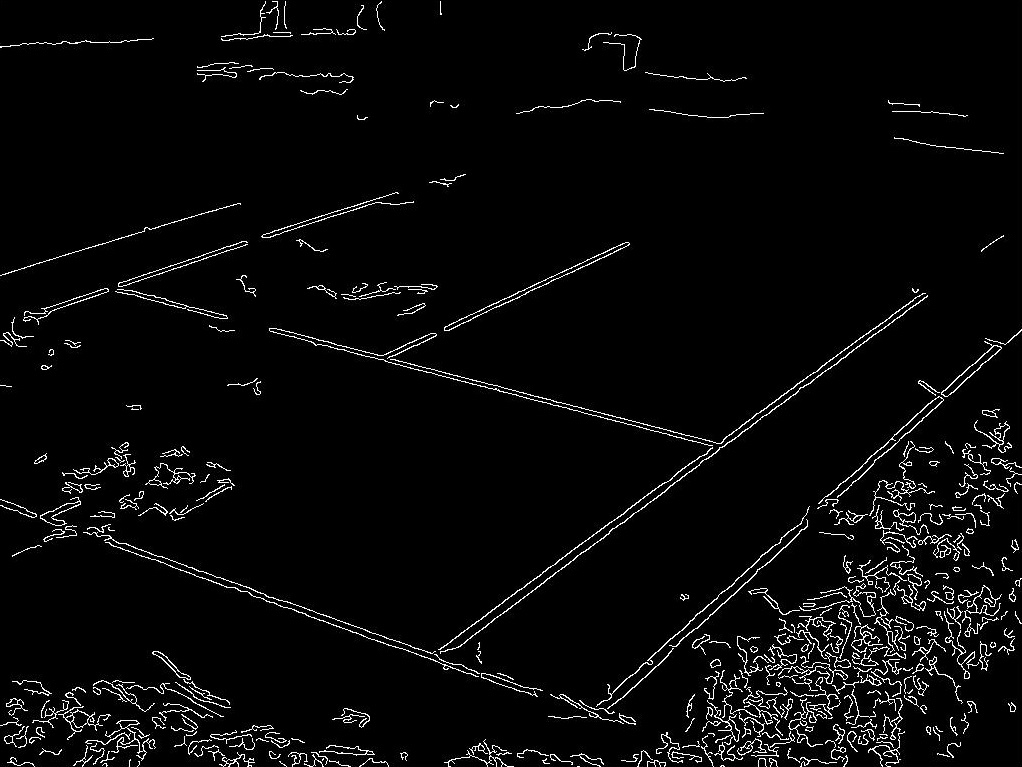
\includegraphics[width=1\textwidth]{4a}
\end{figure}

\noindent
\textbf{4.b} \\
We can find the bounds of the court in the image bu using Hysteresis thresholding. \\
Simply check the maximum value of gradient and use a high threshold to start edge curves and a low
threshold to continue them, and remove everything else that doesn't fit in the category, which includes everything this is below the minimum threshold, and everything above the maximum threshold, and everything that doesn't connect. \\
\end{document}
















